\documentclass{article}
\usepackage[utf8]{inputenc}
\usepackage[spanish.mexico]{babel}
\usepackage[american voltages, american currents,siunitx]{circuitikz}

%para fotos

\usepackage{graphicx}
\usepackage{subcaption}

\title{Previo Práctica 2}
\author{Pablo Vivar Colina \\

}
%\date{Septiembre 2017}

\usepackage{natbib}
\usepackage{graphicx}

\begin{document}

\maketitle

\section{Corriente alterna frente a la continua}

La razón del amplio uso de la corriente alterna viene determinada por su facilidad de transformación, cualidad de la que carece la corriente continua. En el caso de la corriente continua, la elevación de la tensión se logra conectando dínamos en serie, lo que no es muy práctico; al contrario, en corriente alterna se cuenta con un dispositivo, el transformador, que permite elevar la tensión de una forma eficiente.\citep{CA}\\

La energía eléctrica viene dada por el producto de la tensión, la intensidad y el tiempo. Dado que la sección de los conductores de las líneas de transporte de energía eléctrica depende de la intensidad, mediante un transformador se puede elevar la tensión hasta altos valores (alta tensión), disminuyendo en igual proporción la intensidad de corriente. Con esto la misma energía puede ser distribuida a largas distancias con bajas intensidades de corriente y, por tanto, con bajas pérdidas por causa del efecto Joule y otros efectos asociados al paso de corriente, tales como la histéresis o las corrientes de Foucault. Una vez en el punto de consumo o en sus cercanías, el voltaje puede ser de nuevo reducido para su uso industrial o doméstico y comercial de forma cómoda y segura.\citep{CA}\\


\section{Las matemáticas y la CA sinusoidal}

Algunos tipos de oscilaciones periódicas tienen el inconveniente de no tener definida su expresión matemática, por lo que no se puede operar analíticamente con ellas. Por el contrario, la oscilación sinusoidal no tiene esta indeterminación matemática y presenta las siguientes ventajas:\citep{CA}\\

\begin{itemize}
    \item La función seno está perfectamente definida mediante su expresión analítica y gráfica. Mediante la teoría de los números complejos se analizan con suma facilidad los circuitos de alterna.
    
    \item Las oscilaciones periódicas no sinusoidales se pueden descomponer en suma de una serie de oscilaciones sinusoidales de diferentes frecuencias que reciben el nombre de armónicos. Esto es una aplicación directa de las series de Fourier.
    
    \item Se pueden generar con facilidad y en magnitudes de valores elevados para facilitar el transporte de la energía eléctrica.
    
    \item Su transformación en otras oscilaciones de distinta magnitud se consigue con facilidad mediante la utilización de transformadores.
    
\end{itemize}

\subsection{Oscilación Senoidal}

Una señal senoidal o sinusoidal, $a(t)$, tensión, $v(t)$, o corriente, $i(t)$, se puede expresar matemáticamente según sus parámetros característicos (figura \ref{fig:ondaSenoidal}), como una función del tiempo por medio de la siguiente ecuación:\citep{CA}

\begin{equation}
    a(t)=A_0 \cdot \sin(\omega t + \beta)
\end{equation}
\begin{itemize}
    \item $A_0$ es la ''amplitud'' en [V] o [A] (también llamado ''valor máximo o de pico'')
    
    \item $\omega$  pulsación en radianes/segundo
    
    \item $t$ el tiempo en [s]
    
    \item $\beta$ el ángulo de fase inicial en radianes.
\end{itemize}


Dado que la velocidad angular es más interesante para matemáticos que para ingenieros, la fórmula anterior se suele expresar como:\citep{CA}\\

\begin{equation}
    a(t)=A_0 \cdot \sin(2 \pi f t + \beta)
\end{equation}


donde ''f'' es la frecuencia (Hz) y equivale a la inversa del período $f=\frac{1}{T}$. Los valores más empleados en la distribución son 50 Hz y 60 Hz.\citep{CA}


\begin{figure}[H!]
    \centering
    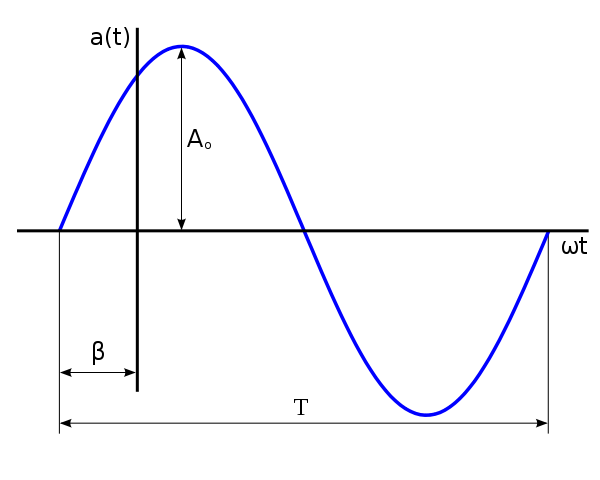
\includegraphics[scale=0.4]{Imagenes/600px-OndaSenoidal.png}
    \caption{Parámetros característicos de una oscilación sinusoidal.}
    \label{fig:ondaSenoidal}
\end{figure}


\section{Amplificador Operacional}

Un amplificador operacional, a menudo conocido op-amp por sus siglas en inglés (operational amplifier) es un dispositivo amplificador electrónico de alta ganancia acoplado en corriente continua que tiene dos entradas y una salida. En esta configuración, la salida del dispositivo es, generalmente, de cientos de miles de veces mayor que la diferencia de potencial entre sus entradas.\citep{AmplificadorOperacional}


\subsection{Comparador}


Aplicación sin retroalimentación que compara señales entre las dos entradas y presenta una salida en función de qué entrada sea mayor. Se puede usar para adaptar niveles lógicos.\citep{AmplificadorOperacional}

\begin{equation}
    {\displaystyle V_{\rm {out}}=\left\{{\begin{matrix}V_{S+}&V_{1}>V_{2}\\V_{S-}&V_{1}<V_{2}\end{matrix}}\right.} 
\end{equation}

Una aplicación simple pero útil, es la de proporcionar un sistema de control ON-OFF. Por ejemplo un control de temperatura, cuya entrada no inversora se conecta un termistor (sensor de temperatura) y en la entrada inversora un divisor resistivo con un preset (resistencia variables) para ajustar el valor de tensión de referencia. Cuando en la pata no inversora exista una tensión mayor a la tensión de referencia, la salida activara alguna señalización o un actuador.\citep{AmplificadorOperacional}

\subsection{Seguidor de Voltaje o tensión}

Es aquel circuito que proporciona a la salida la misma tensión que a la entrada. Presenta la ventaja de que la impedancia de entrada es elevada, la de salida prácticamente nula, y es útil como un buffer, para eliminar efectos de carga o para adaptar impedancias (conectar un dispositivo con gran impedancia a otro con baja impedancia y viceversa) y realizar mediciones de tensión de un sensor con una intensidad muy pequeña que no afecte sensiblemente a la medición.\citep{AmplificadorOperacional}

\begin{figure}[h!]
    \centering
    \includegraphics[width=0.5\textwidth]{Imagenes/Buffer.png}
    \caption{Amplificador operacional en modo seguidor de tensión \citep{AmplificadorOperacional}}
    \label{fig:buffer}
\end{figure}

\subsection{Amplificador no inversor}

En el modo amplificador no inversor, el voltaje de salida cambia en la misma dirección del voltaje de entrada.\citep{AmplificadorOperacional}

La ecuación de ganancia para esta configuración es:

\begin{equation}
    {\displaystyle V_{\text{out}}=A_{OL}\,(V_{\!+}-V_{\!-})} 
\end{equation}

Sin embargo, en este circuito $V−$ es una función de $V_{out}$ debido a la realimentación negativa a través de la red constituida por $R1$ y $R2$, donde $R1$ y 
$R2$ forman un divisor de tensión, y como V− es una entrada de alta impedancia, no hay efecto de carga. Por consiguiente:

\begin{equation}
    {\displaystyle V_{\!-}\,\,=\beta \cdot V_{\text{out}}} 
\end{equation}


Donde:

\begin{equation}
{\displaystyle \beta ={\frac {R_{1}}{R_{1}+R_{2}}}}
\end{equation}

Sustituyendo esto en la ecuación de ganancia, se obtiene:


\begin{equation}
{\displaystyle V_{\text{out}}=A_{OL}(V_{\text{in}}-\beta \cdot V_{\text{out}})}
\end{equation}


Resolviendo para ${\displaystyle V_{\text{out}}} {\displaystyle V_{\text{out}}}:$

\begin{equation}
{\displaystyle V_{\text{out}}=V_{\text{in}}\left({\frac {1}{\beta +1/A_{OL}}}\right)} 
\end{equation}


Si ${\displaystyle A_{OL}} {\displaystyle A_{OL}}$ es muy grande, se simplifica a



\begin{equation}
{\displaystyle V_{\text{out}}\approx {\frac {V_{\text{in}}}{\beta }}={\frac {V_{\text{in}}}{\frac {R_{\text{1}}}{R_{\text{1}}+R_{\text{2}}}}}=V_{\text{in}}\left(1+{\frac {R_{2}}{R_{1}}}\right)}
\end{equation}

\begin{figure}[h!]
    \centering
    \includegraphics[width=0.5\textwidth]{Imagenes/Opampintegrating.png}
    \caption{Amplificador operacional en modo no inversor\citep{AmplificadorOperacional}}
    \label{fig:OpAmpInvert}
\end{figure}

\subsection{Sumador inversor}

Aplicación en la cual la salida es de polaridad opuesta a la suma de las señales de entrada.\citep{AmplificadorOperacional}\\

Para resistencias independientes $R1, R2,... Rn
$

\begin{equation}
{\displaystyle V_{\mathrm {out} }=-R_{f}\left({\frac {V_{1}}{R_{1}}}+{\frac {V_{2}}{R_{2}}}+\dots +{\frac {V_{n}}{R_{n}}}\right)}
\end{equation}

La expresión se simplifica bastante si se usan resistencias del mismo valor
Impedancias de entrada: $Zn = Rn$\citep{AmplificadorOperacional}\\

\begin{figure}
    \centering
    \includegraphics[width=0.5\textwidth]{Imagenes/Opampsumming.png}
    \caption{Amplificador sumador de n entradas.\citep{AmplificadorOperacional}}
    \label{fig:opAmpSumming}
\end{figure}


\subsection{Restador Inversor}

Para resistencias independientes R1,R2,R3,R4 la salida se expresa como:\citep{AmplificadorOperacional}

\begin{equation}[h!]
    {\displaystyle V_{\mathrm {out} }=V_{2}\left({\left(R_{3}+R_{1}\right)R_{4} \over \left(R_{4}+R_{2}\right)R_{1}}\right)-V_{1}\left({R_{3} \over R_{1}}\right)}
\end{equation}

La impedancia diferencial entre dos entradas es:

\begin{equation}
{\displaystyle Z_{\rm {in}}=R_{1}+R_{2}+R_{\rm {in}}}
\end{equation}

donde ${\displaystyle R_{in}}$ ${\displaystyle R_{in}}$ representa la resistencia de entrada diferencial del amplificador, ignorando las resistencias de entrada del amplificador de modo común. Este tipo de configuración tiene una resistencia de entrada baja en comparación con otro tipo de restadores como el amplificador de instrumentación.\citep{AmplificadorOperacional}

\begin{figure}[h!]
    \centering
    \includegraphics[width=0.5\textwidth]{Imagenes/Opampdifferencing.png}
    \caption{Amplificador restador-inversor\citep{AmplificadorOperacional}}
    \label{fig:my_label}
\end{figure}



%\begin{figure}
 %   \centering
  %  \includegraphics{Imagenes/OpAmpLazoAbierto.png}
   
   % \caption{Amplificador operacional en modo de lazo abierto, configuración usada como comparador.}
    %\label{fig:opAmpLazoAbierto}
%\end{figure}



\subsection{Amplificador Ideal}

\begin{figure}
    \centering
    \includegraphics[width=0.5\textwidth]{Imagenes/OpAMpIdeal.png}
    \caption{Circuito equivalente de un amplificador operacional\citep{AmplificadorOperacional}}
    \label{fig:opAmpIdeal}
\end{figure}




%\section{Circuito a resolver}

%\begin{figure}[h!]
 %   \centering
   % \includegraphics{}
  %  \begin{circuitikz}
%\draw

%(-1,0)--(-1,-1)
%(-1,-1) to[V,l=$28v$](-1,-2) 
% (-1,-2)--(-1,-3)
 
 %(-1,-3)--(2,-3)
 
% (-1,0) to[R,l=$50 \Omega $](2,0)
 
 
% (2,-3)to[R,l=$5 \Omega$](2,0)
 
% (2,0)--(4,0)
% (2,-3)--(4,-3)
 
 % (4,-3)to[R,l=$10 \Omega$](4,0)
 
 
%;

%\draw[thick,arrows=->]
%(2.5,0)--(2.5,-1)
%;
 
%\end{circuitikz}
 %   \caption{Circuito a resolver}
  %  \label{fig:circuito}
%\end{figure}

%\subsection{Resultados}

%Para resolver el circuito se hicieron equivalente los resistores de 5 y 10 $\Omegas$ para obtener el voltaje en esas ramas, así se pudo deducir la corriente en la rama del resistor de 50 $\Omega$ y el circuito equivalente, posterirmente se usaron las leyes de Kirchhoff para deducir los voltajes y las corrientes respectivamente.

%\begin{table}[h!]
%\centering

%\begin{tabular}{|c|c|c|}
%\hline
%Componente & V {[}V{]} & I {[}A{]} \\ \hline
%R 50       & 26.25     & 0.525     \\ \hline
%R 10       & 1.75      & 0.173     \\ \hline
%R 5        & 1.75      & 0.352     \\ \hline
%V fuente   & 28        & 0.525     \\ \hline
%\end{tabular}
%\caption{Tabla de Resultados}
%\label{tabla-resultados}

%\end{table}

%.\\[100cm]
\bibliographystyle{plain}
\bibliography{Referencias.bib}


\end{document}